% Chapter 2

\chapter{Project 2a: Matrix multiplication} % Main chapter title

\label{Chapter2} % for referencing this chapter elsewhere, use \ref{Chapter2}

\lhead{Chapter 2. \emph{Matrix multiplication}} % this is for the header on each page - perhaps a shortened title

%----------------------------------------------------------------------------------------


\section{Introduction}



\section{Implementations \citep{matrixMultiplication}}


\subsection{Naive Matrix Multiplikation}
We have implemented a naive matrix multiplication to compare with the other algorithms.

The first line creates a matrix for saving the result of the multiplication in.

Then for all the rows in the first matrix and all the colums in the second matrix we take sum of the row element multiplied with the column element for alle the elements in the current column and row.

Then we save the value in the resulting matrix.
After we have iterated trough all the columns and rows we return the resulting matrix.
\lstinputlisting[language=C++, firstline=16, lastline=29, numbers=left]{./Figures/Project2a/NaiveMatrixMulti.cpp}

\subsection{Transposed}
\lstinputlisting[language=C++, firstline=5, lastline=6, numbers=left]{./Figures/Project2a/Transpose.cpp}
We start by transposing the input matrix in a transpose method that is called in the setup method.
\lstinputlisting[language=C++, firstline=12, lastline=14, numbers=left]{./Figures/Project2a/Transpose.cpp}
The setup method should always be called before the matrix multiplication method is used.
\lstinputlisting[language=C++, firstline=16, lastline=26, numbers=left]{./Figures/Project2a/Transpose.cpp}
After the transpose method has been called we start by creating a matrix p we use to save the result in.
Then for all the colums in the transposed matrix mC, and all the colums in the second matrix B, we calculate the sum of the product between all the enties in the current column of mC and B.
When we have iterated through all the colums in both matrixes and saved the results we are done.
\lstinputlisting[language=C++, firstline=29, lastline=42, numbers=left]{./Figures/Project2a/Transpose.cpp}


\subsection{Recursive}
The recursive multiplication is implemented as follows:
\begin{verbatim}
   int m = heightA;
  int n = widthA;
  int p = (*matrixB).nCols;
  B = matrixB;
  C = createMatrix(m, p);
  
  recMult(0, 0, 0, 0, m, n, p);
  
  return C;
\end{verbatim}

It makes use of the following recursive method:
\begin{verbatim}
void recMult(int i_A, int j_A, int i_B, int j_B, int m, int n, int p) {
  if (m==1 && n==1 && p==1) { // base case
    int AB = matrixGet(A, i_A, j_A)*matrixGet(B, i_B, j_B);
    matrixAdd(C, i_A, j_B, AB);
  } else if (m >= max(n,p)) { // split rows of A
    recMult(i_A,     j_A,     i_B,     j_B,     m/2,   n,     p    );
    recMult(i_A+m/2, j_A,     i_B,     j_B,     m-m/2, n,     p    );
  } else if (n >= max(m,p)) { // split columns of A and rows of B
    recMult(i_A,     j_A,     i_B,     j_B,     m,     n/2,   p    );
    recMult(i_A,     j_A+n/2, i_B+n/2, j_B,     m,     n-n/2, p    );
  } else if (p >= max(m,n)) { // split columns of B
    recMult(i_A,     j_A,     i_B,     j_B,     m,     n,     p/2  );
    recMult(i_A,     j_A,     i_B,     j_B+p/2, m,     n,     p-p/2);
  }
  return;
}
\end{verbatim}



\subsection{Tiled}
The implementation of tiled matrix multiplication (TMM) is based on \citep{matrixMultiplication}, where TMM is presented as an example of an cache-aware algorithm. 
The approach is to multiply two matrices by dividing them into sub-matrices and multiplying these. 
\begin{figure}[htbp]
	\centering
		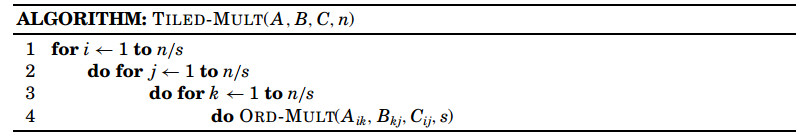
\includegraphics[width=\textwidth]{./Figures/Project2a/TiledMulti_Pseudo.jpg}
		\rule{35em}{0.5pt}
	\caption[Branch misses]{
	Bla bla bla.
	}
	\label{fig:Branch_misses}
\end{figure}
The idea is to base the size of the sub-matrices on the cache size and thereby utilize the cache in the best way (i.e. fewer cache faults).   

TMM is implemented by splitting the input matrices (A and B) into S sub-matrices in each dimension, then multiplying the sub-matrices producing the multiplied matrix (C). 
The value of S is calculated based on a value \verb!CACHE_SIZE_KB! which we choose depending on the platform. S is calculated so that three sub-matrices can fit in cache at the same time (as described in the article).
The calculation is as follows:
\begin{lstlisting}[numbers=left]
  ...
  // Needs to be 3 sub mats in cache at a time
  int allowedSizeOfSubMat = (CACHE_SIZE_KB*1024) / 3;
  int numOfSubMats = allowedSizeOfSubMat / sizeof(int);
  s = ceil( sqrt(numOfSubMats) );
  ... 
\end{lstlisting}
The multiplication of the sub-matrices is calculated with the naive matrix multiplication method. 
The biggest challenge in the implemtation was to seperate the input matrices int sub-matrices without actually creating new matrices, which would use a lot of extra memory and computation time. 
Instead we keep track of the start indices of the sub-matrices and just access A and B to get the values. 
To keep track of how far we have gotten in each direction in A and B and how big the next sub-matrices is, we maintain six variables:
\begin{lstlisting}[numbers=left]
  ...
  int subAnRows, subAnCols, subBnCols;
  int rowsVisitedA = 0;
  int colsVisitedA = 0;
  int colsVisitedB = 0;
  ...
\end{lstlisting}
The size of the new sub-matrix (e.g. subAnRows) are updated each time we iterate in the corresponding direction (e.g. rows). 
The new value depends on how far we've gotten and the size of the input e.g.
\begin{lstlisting}
subAnRows = ceil( (double) (A->nRows - rowsVisitedA) / (double) (s - i) );
\end{lstlisting}

We only need three variables to maintain where we are in A, B and C, and not four, because of the constraint that A has to have as many coloumns as B has rows for the two to be multiplied. 
Maintaining these values also means that A and B can be multiplied without depending on that they are symmetric or have the same size, as long as they comply with forementioned constraint.



\section{Results and discussion}



\begin{figure}[htbp]
	\centering
		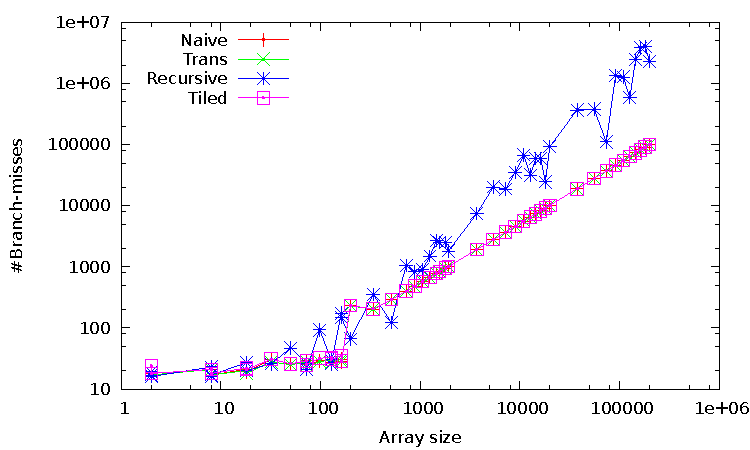
\includegraphics[width=\textwidth]{./Figures/Project2a/Branch_misses.pdf}
		\rule{35em}{0.5pt}
	\caption[Branch misses]{
	Bla bla bla.
	}
	\label{fig:Branch_misses}
\end{figure}


\begin{figure}[htbp]
	\centering
		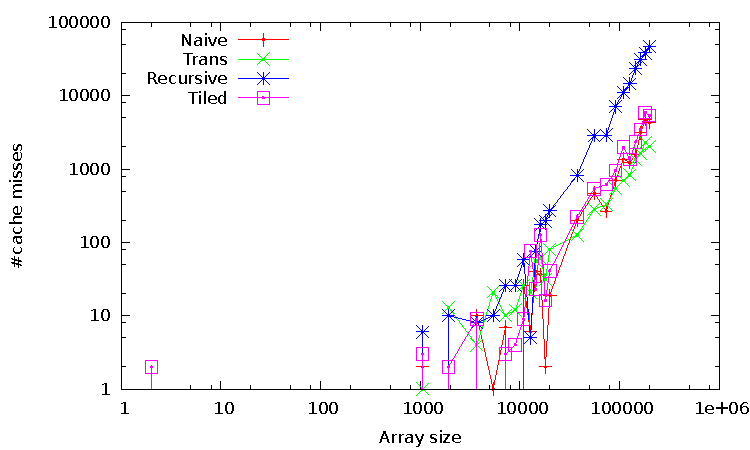
\includegraphics[width=\textwidth]{./Figures/Project2a/Cache_misses.pdf}
		\rule{35em}{0.5pt}
	\caption[Cache misses]{
	Bla bla bla.
	}
	\label{fig:Cache_misses}
\end{figure}



\begin{figure}[htbp]
	\centering
		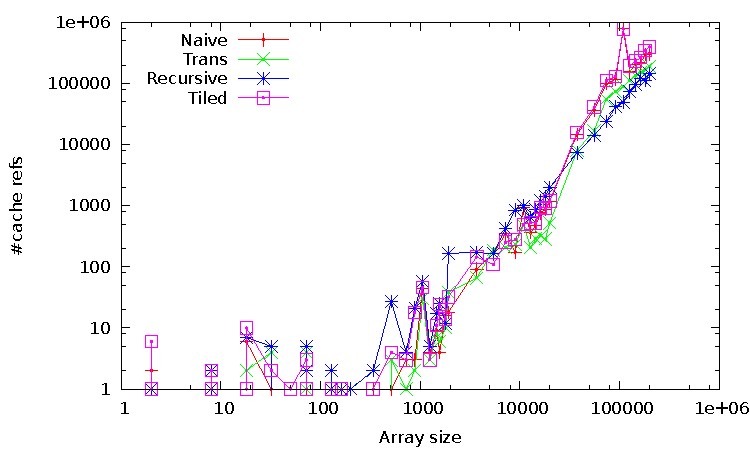
\includegraphics[width=\textwidth]{./Figures/Project2a/Cache_refs.pdf}
		\rule{35em}{0.5pt}
	\caption[Cache refs]{
	Bla bla bla.
	}
	\label{fig:Cache_refs}
\end{figure}



\begin{figure}[htbp]
	\centering
		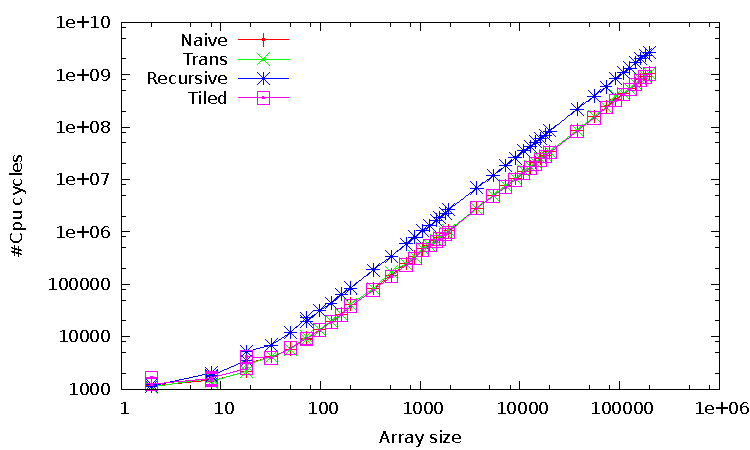
\includegraphics[width=\textwidth]{./Figures/Project2a/Cpu_cycles.pdf}
		\rule{35em}{0.5pt}
	\caption[CPU cycles]{
	Bla bla bla.
	}
	\label{fig:Cpu_cycles}
\end{figure}


\begin{figure}[htbp]
	\centering
		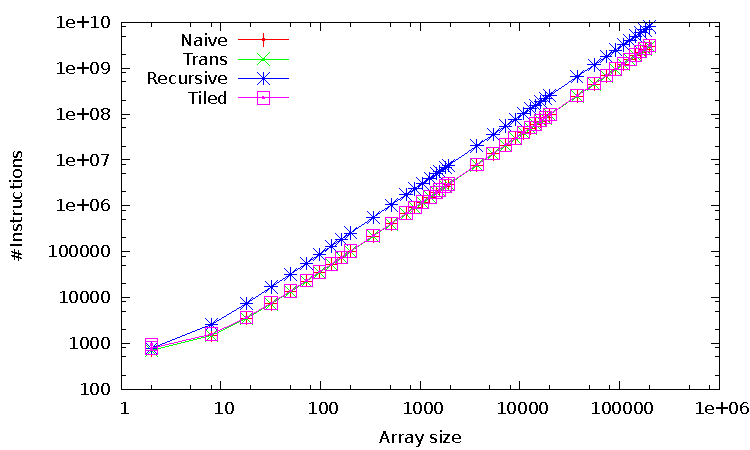
\includegraphics[width=\textwidth]{./Figures/Project2a/Instructions.pdf}
		\rule{35em}{0.5pt}
	\caption[Instructions]{
	Bla bla bla.
	}
	\label{fig:Instructions}
\end{figure}
